\chapter{Problematyka zagadnienia}
\label{ch:problematyka}

%---------------------------------------------------------------------------
\section{Charakterystyka choroby Parkinsona}
\label{sec:charakterystykaPD}

Choroba Parkinsona (PD) jest zwyrodnieniowym schorzeniem mózgu związanym z objawami motorycznymi (spowolnienie ruchowe,
drżenie, sztywność, zaburzenia chodu i równowagi) oraz szeroką gamą powikłań niemotorycznych (zaburzenia poznawcze,
zaburzenia psychiczne, zaburzenia snu oraz ból i inne zaburzenia sensoryczne).
Objawy zwykle zaczynają się stopniowo i nasilają z czasem.
Ich postęp powoduje wysoki stopień niepełnosprawności i konieczność opieki.
U wielu osób z PD w trakcie trwania choroby mogą również rozwinąć się zmiany psychiczne i behawioralne, problemy ze snem,
depresja, problemy z pamięcią i zmęczenie.


Przyczyna PD nie jest znana, ale uważa się, że powstaje w wyniku złożonej interakcji pomiędzy czynnikami genetycznymi i
narażeniem na czynniki środowiskowe, takie jak pestycydy, rozpuszczalniki i zanieczyszczenia powietrza.
Niektóre przypadki PD wydają się być dziedziczne, a kilka przypadków można przypisać określonym wariantom genetycznym.
Chociaż uważa się, że genetyka odgrywa rolę w chorobie Parkinsona, w większości przypadków choroba nie występuje rodzinnie\cite{National_Institute_on_Aging_2022}.

\begin{figure}[htbp]
	\centering
	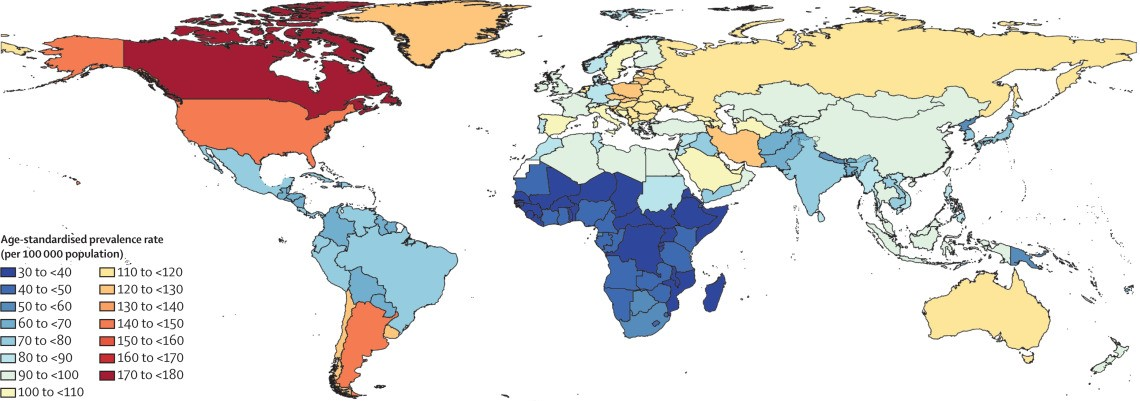
\includegraphics[width=0.9\textwidth]{./img/map}
	\caption{Choroba Parkinsona na świecie \cite{global_PD}}
    \label{fig:PD_map}
\end{figure}

Według raportu Światowej Organizacji Zdrowia\cite{WHO} w skali globalnej niepełnosprawność i zgony z powodu PD
rosną szybciej niż w przypadku jakichkolwiek innych zaburzeń neurologicznych.
Częstość występowania PD podwoiła się w ciągu ostatnich 25 lat.
Globalne szacunki w 2019 roku wykazały ponad 8,5 miliona osób z PD.
Obecne szacunki sugerują, że w 2019 roku PD spowodowała 5,8 miliona lat życia z niepełnosprawnością, co
stanowi wzrost o 81\% od 2000 roku, i spowodowała 329 000 zgonów, co stanowi wzrost o ponad 100\% od 2000 roku.

W Polsce z chorobą Parkinsona zmaga się około 100 tys. pacjentów, z czego około 20\% jest już w stadium zaawansowanym
według informacji przekazywanych przez Fundację Chorób Mózgu.
Ponadto co roku w naszym kraju wykrywanych jest ok. 8 tys. nowych zachorowań.
Nowe zachorowania nadal skorelowane są z wiekiem, średnia wieku chorych wynosi 60 lat, niestety wzrasta odsetek chorych wśród osób młodych (nawet w wieku 20 lat).

Chociaż każdy może być narażony na ryzyko rozwoju choroby Parkinsona, badania naukowe sugerują,
że choroba ta dotyka więcej mężczyzn niż kobiet.
Statystyki pokazują, że ryzyko zachorowania rośnie wraz z wiekiem, chociaż choroba może dotyczyć także młodszych osób.
U większości osób z PD po raz pierwszy choroba rozwija się po 60 roku życia, około 5\% do 10\% doświadcza jej początku przed 50 rokiem życia.
Postacie choroby Parkinsona o wczesnym początku są często, choć nie zawsze, dziedziczne i niektóre formy zostały powiązane z
określonymi zmianami w genach\cite{National_Institute_on_Aging_2022}.

\begin{figure}[htbp]
	\centering
	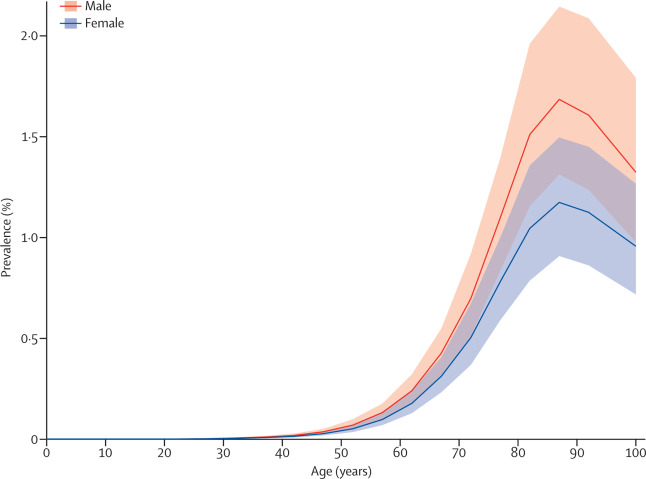
\includegraphics[width=0.6\textwidth]{./img/PD_prevalence}
	\caption{Rozpowszechnienie choroby Parkinsona w zależności od wieku \cite{global_PD}}
    \label{fig:PD_prevalance}
\end{figure}

%---------------------------------------------------------------------------

\subsection{Objawy choroby}
\label{subsec:objawy}

Najbardziej widoczne oznaki i objawy choroby Parkinsona pojawiają się, gdy komórki nerwowe w zwojach podstawy mózgu,
obszarze mózgu kontrolującym ruch, ulegają uszkodzeniu i/lub obumierają.
Zwykle te komórki nerwowe lub neurony wytwarzają dopaminę.
Kiedy neurony obumierają lub ulegają uszkodzeniu, wytwarzają mniej dopaminy, co powoduje problemy z poruszaniem się
związane z chorobą.
Na ten moment nie wiadomo co powoduje śmierć neuronów.
Zanikają również zakończenia nerwowe, które wytwarzają norepinefrynę, główny przekaźnik chemiczny
współczulnego układu nerwowego, który kontroluje wiele funkcji organizmu, takich jak tętno i ciśnienie krwi.
Utrata norepinefryny może pomóc wyjaśnić niektóre cechy choroby Parkinsona związane z brakiem ruchu, takie jak zmęczenie,
nieregularne ciśnienie krwi, zmniejszony ruch pokarmu w przewodzie pokarmowym i nagły spadek ciśnienia krwi, gdy osoba wstaje z pozycji siedzącej lub leżącej.


Do czterech głównych objawów choroby Parkinsona zalicza się:
\begin{itemize}[itemsep=0.5pt]
	\item Drżenie rąk, ramion, nóg, szczęki lub głowy
	\item Sztywność mięśni, gdy mięśnie pozostają skurczone przez długi czas
	\item Powolność ruchu
	\item Zaburzenia równowagi i koordynacji, czasami prowadzące do upadków
\end{itemize}


Pozostałe objawy mogą obejmować:
\begin{itemize}[itemsep=0.5pt]
	\item Depresja i inne zmiany emocjonalne
	\item Trudności w połykaniu, żuciu i mówieniu
	\item Problemy z układem moczowym lub zaparcia
	\item Problemy skórne
\end{itemize}

Objawy choroby Parkinsona i tempo progresji różnią się u poszczególnych osób.
Początkowo są subtelne i pojawiają się stopniowo.
Często zaczynają się po jednej stronie ciała lub nawet w jednej kończynie.
W miarę postępu choroby ostatecznie dotyka ona obu stron, jednak objawy mogą być bardziej nasilone po jednej stronie niż po drugiej.
Wiele osób z chorobą Parkinsona zauważa, że przed wystąpieniem sztywności i drżenia miały problemy ze snem, zaparcia, utratę węchu oraz zespół niespokojnych nóg.
Należy pamiętać, że niektóre z tych objawów mogą również wystąpić podczas normalnego starzenia się \cite{National_Institute_on_Aging_2022}.

%---------------------------------------------------------------------------

\subsection{Etapy choroby}
\label{subsec:etapy}

Tu będę opierać się na tym\cite{Szurek_2018} i na tym\cite{Wieczorek_2013} i na tym\cite{Kuryłowicz_2019}

Wielu lekarzy, którzy diagnozują to zaburzenie mózgu, polega na skali oceny Hoehna i Yahra, aby sklasyfikować nasilenie objawów.
Skala jest podzielona na pięć etapów w zależności od postępu choroby.
Pięć etapów pomaga lekarzom ocenić, jak daleko zaawansowana jest choroba.

W praktyce klinicznej często dodaje się stopnie pośrednie (1,5, 2,5, 3,5 i 4,5), które spełniają kryteria stopnia niższego, ale obecne są (niestale lub w niewielkim nasileniu) objawy kwalifikujące do stopnia wyższego.

\begin{itemize}[itemsep=0.5pt]
	\item Etap 0.0: Brak objawów choroby
	\item Etap 1.0: Łagodny: objawy parkinsonowskie tylko po jednej stronie ciała
	\item Etap 1.5: Objawy jednostronne i osiowe.
	\item Etap 2.0: Objawy po obu stronach ciała (zwykle z przewagą jednej z nich), bez zaburzeń równowagi
	\item Etap 2.5: Łagodne obustronne zajęcie z powrotem do zdrowia w teście retropulsacji (pull).
	\item Etap 3.0: Zaburzenia równowagi, łagodna lub średnio zaawansowana choroba, niezależność w zakresie samoobsługi
	\item Etap 4.0: Ciężka niepełnosprawność, jednak chory jest w stanie poruszać się i utrzymywać postawę stojącą bez pomocy innych osób
	\item Etap 5.0: Chory wymaga wózka inwalidzkiego lub jest całkowicie unieruchomiony w łóżku
\end{itemize}

[https://www.parkinson.org/understanding-parkinsons/what-is-parkinsons/stages]
Jedną z krytyki skali Hoehna i Yahra jest fakt, że skupia się ona wyłącznie na kwestiach związanych z ruchem i wynikającymi z niego problemami. Jednak inne objawy są związane z PD, takie jak różne formy zmian poznawczych i upośledzenia, w tym początek stanów, takich jak zaburzenia zachowania podczas snu REM.

Z tego powodu niektórzy lekarze wybierają alternatywę, zunifikowaną skalę oceny choroby Parkinsona MDS. Skala ta składa się z pięćdziesięciu kompleksowych pytań służących do analizy objawów motorycznych i niemotorycznych w celu uzyskania szerszego spojrzenia na trudności pacjenta.
Ich odkrycia mogą pomóc w ocenie upośledzeń funkcji poznawczych, które utrudniają codzienne zadania, obok problemów z poruszaniem się, w oferowaniu skuteczniejszych form leczenia.
Chociaż jest bardziej złożony, zapewnia lekarzom dokładniejszy wgląd w specyficzne upośledzenia i potrzeby danej osoby. Dysponując większą wiedzą i danymi, lekarze uzyskują pełniejszy obraz stanu psychicznego i fizycznego danej osoby, a nie tylko jej zdolności motorycznych.

Do wczesnych objawów choroby Parkinsona zalicza się [https://www.parkinson.org/understanding-parkinsons/what-is-parkinsons/stages]:
\begin{itemize}[itemsep=0.5pt]
	\item drżenie palców, kciuków, dłoni lub podbródka
	\item drobne lub stłoczone pismo odręczne
	\item utrata węchu
	\item problemy ze snem
	\item problemy z poruszaniem się lub chodzeniem
	\item zaparcie
	\item miekki lub niski głos
	\item zamaskowan twarz
	\item zawroty głowy i omdlenia
	\item pochylanie się lub garbienie się
\end{itemize}

%---------------------------------------------------------------------------

\subsection{Terapia osób chorych}
\label{subsec:terapia}
Aktualnie nie istnieje lekarstwo na chorobę Parkinsona, dlatego leczenie PD skupia się na przywróceniu pacjentowi sprawności
lub w bardzo zaawansowanych przypadkach przynajmniej poprawę życia.
Zgodnie z aktualną praktyką medyczną wyróżnia się następujące metody terapii \cite{National_Institute_on_Aging_2022}:

\renewcommand{\labelenumi}{\alph{enumi})}
\begin{enumerate}
	\item Leczenie farmakologiczne

Zasada działania większości ze stosowanych leków opiera się na zwiększeniu poziomu dopaminy w mózgu.
Wpływa ona na inne substancje chemiczne w mózgu, takie jak neuroprzekaźniki, które przekazują informacje między komórkami mózgowymi.
Dzięki temu pomaga kontrolować objawy niezwiązane z ruchem.
Główną terapią choroby Parkinsona jest lewodopa.
Komórki nerwowe wykorzystują lewodopę do wytwarzania dopaminy w celu uzupełnienia kurczących się zasobów mózgu.
Zwykle ludzie przyjmują lewodopę razem z innym lekiem zwanym karbidopą.
Karbidopa zapobiega lub zmniejsza niektóre skutki uboczne leczenia lewodopą - takie jak nudności, wymioty, niskie ciśnienie
krwi i niepokój - oraz zmniejsza ilość lewodopy potrzebną do złagodzenia objawów.
Oprócz tego stosowane są leki o innym działaniu:

\begin{itemize}[itemsep=0.5pt]
	\item agoniści dopaminy stymulujący produkcję dopaminy w mózgu
	\item inhibitory enzymów (np. inhibitory MAO-B, inhibitory COMT) w celu zwiększenia ilości dopaminy poprzez spowolnienie enzymów rozkładających dopaminę w mózgu
	\item amantadyna, aby pomóc zmniejszyć ruchy mimowolne
	\item leki antycholinergiczne zmniejszające drżenie i sztywność mięśni
\end{itemize}


	\item Głeboka stymulacja mózgu
	
W przypadku osób z chorobą Parkinsona, które nie reagują dobrze na leki, lekarz może zalecić Głęboką Stymulację Mózgu (ang. Deep Brain Stimulation, w skrócie - DBS). Podczas zabiegu chirurgicznego lekarz wszczepia elektrody do części mózgu i łączy je z małym urządzeniem elektrycznym wszczepionym w klatkę piersiową. Urządzenie i elektrody bezboleśnie stymulują określone obszary w mózgu kontrolujące ruch w sposób, który może pomóc w zatrzymaniu wielu objawów choroby Parkinsona związanych z ruchem, takich jak drżenie, spowolnienie ruchu i sztywność.

	\item Rehabilitacja

Rehabilitacja neurologiczna przy chorobie Parkinsona jest niezwykle ważna. Powinna towarzyszyć pacjentowi już od postawienia diagnozy.  Mogą one pomóc w zaburzeniach chodu i głosu, drżeniach i sztywności oraz pogorszeniu funkcji umysłowych. Wśród przykładowych terapii można wyróżnić:
zdrowa dieta wspierająca ogólne samopoczucie
ćwiczenia wzmacniające mięśnie i poprawiające równowagę, elastyczność i koordynację
masaż leczniczy redukujący napięcie
joga i tai chi w celu zwiększenia rozciągania i elastyczności
rehabilitacja foniczna, eliminująca trudności w mówieniu
psychoterapia, potrzebna wielu pacjentom, aby mogli się cieszyć pełnią życia.
\end{enumerate}

Chociaż postęp choroby Parkinsona jest zwykle powolny, ostatecznie może to wpłynąć na codzienne czynności danej osoby. Czynności takie jak praca, zajmowanie się domem i udział w zajęciach towarzyskich z przyjaciółmi mogą stać się wyzwaniem. Doświadczanie tych zmian może być trudne, ale grupy wsparcia mogą pomóc ludziom sobie z tym poradzić. Grupy te mogą dostarczać informacji, porad i łączy z zasobami dla osób żyjących z chorobą Parkinsona, ich rodzin i opiekunów.

%---------------------------------------------------------------------------

\subsection{Metody diagnozowania i monitorowania choroby Parkinsona}
\label{subsec:diagnostyka}

Ile czasu potrzeba w praktyce klinicznej, aby postawić diagnozę klinicznie potwierdzonej choroby Parkinsona?\cite{ROSSI202153}

• Empirycznie zaproponowano ramy czasowe od 3 do 10 lat, aby postawić diagnozę klinicznie potwierdzonej choroby Parkinsona.

• U pacjentów z parkinsonizmem zbadano czas do ostatecznej diagnozy klinicznej oraz czynniki przewidujące szybsze rozpoznanie.

• Potrzebne były trzy lata w warunkach klinicznych, aby zdiagnozować 95 procent pacjentów, u których początkowo występował parkinsonizm.

• Szybsze diagnozy postawiono u pacjentów z pozytywną odpowiedzią na lewodopę.

Wdrożenie przyjętych klinicznych kryteriów diagnostycznych poprawiło dokładność diagnozy klinicznej choroby Parkinsona (PD). Empirycznie zaproponowano ramy czasowe od 3 do 10 lat, aby postawić diagnozę klinicznie potwierdzonej PD.
Zbadaliśmy czas do ostatecznej diagnozy klinicznej (FCD) i czynniki, które przewidują szybsze rozpoznanie u pacjentów z
parkinsonizmem i/lub drżeniem w latach 2009-2015 w naszym ośrodku trzeciego stopnia.
Wszyscy pacjenci przeszli wystandaryzowany proces treningu w celu osiągnięcia FCD, który obejmował ostrą prowokację lewodopą (LDC) po pierwszej wizycie.
Spośród 326 włączonych pacjentów, 215 (66\%) otrzymało FCD w ciągu pierwszych sześciu miesięcy po LDC. FCD osiągnięto u 95\% i 100\% pacjentów odpowiednio po 33 i 108 miesiącach. ChP była FCD u 196 pacjentów (60,1\%). FCD osiągano szybciej u pacjentów z pozytywną odpowiedzią na lewodopę oraz gdy FCD była PD.
Czas potrzebny do postawienia ostatecznego rozpoznania w warunkach klinicznych wynosił 2,75 roku u 95\% pacjentów, u których
początkowo występował parkinsonizm i/lub drżenie. Pacjenci z pozytywną odpowiedzią na lewodopę w LDC skorzystali z krótszych opóźnień do FCD.


Diagnostyka różnicowa choroby Parkinsona (PD) obejmuje atypowy parkinsonizm neurodegeneracyjny, taki jak zanik wieloukładowy (MSA),
postępujące porażenie nadjądrowe (PSP), zespół korowo-podstawny (CBS) i otępienie z ciałami Lewy'ego (DLB), jak również inne stany niezwyrodnieniowe,
takie jak drżenie samoistne, parkinsonizm polekowy, parkinsonizm naczyniowy i wodogłowie normalnego ciśnienia.
Chociaż ostateczną diagnozę można postawić jedynie na podstawie autopsji mózgu, diagnozę kliniczną można uzyskać,
stosując wcześniej zdefiniowane kryteria diagnostyczne, takie jak kryteria Banku Mózgu Brytyjskiego Towarzystwa Choroby Parkinsona (UKPDSBB)
oraz ostatnio opracowane Międzynarodowe Kliniczne kryteria diagnostyczne choroby Parkinsona (ang. Movement Disorders Society, MDS).
Ostatnie dane sugerują, że ta ostatnia ma ogólną dokładność dla prawdopodobnego PD na poziomie 92,6\%.
Dla pacjentów z chorobą trwającą krócej niż 5 lat swoistość klinicznie prawdopodobnego rozpoznania PD wynosiła 87\%.
Zarówno kryteria UKPDSBB, jak i MDS Clinical Diagnostic Criteria for PD proponują ramy czasowe 3, 5, a nawet 10 lat,
podczas których wykrycie niektórych klinicznych aspektów choroby pozwoliłoby na postawienie jednoznacznego rozpoznania klinicznie potwierdzonej PD.
Takie ramy czasowe zostały ustalone na podstawie empirycznych i niesystematycznych dowodów.
Dla celów badawczych niedawno zaproponowano koncepcję klinicznie potwierdzonej „wczesnej PD” w oparciu o zmodyfikowaną wersję kryteriów MDS,
usuwając wszystkie składowe czasu trwania choroby i zmieniając czerwone flagi na bezwzględne wykluczenia, wykazując swoistość 95,4\%.
Badanie kliniczno-patologiczne wykazało, że dokładność klinicznego rozpoznania PD wynosiła zaledwie 53\% u pacjentów z chorobą trwającą krócej
niż 5 lat i odpowiedzią na dopaminową terapię zastępczą, która wzrosła do 88\% po ponad 5 latach trwania choroby. Co więcej,
dokładność klinicznego rozpoznania PD u osób nieleczonych lub niereagujących wyraźnie na chorobę Parkinsona wynosiła tylko 26\%, co
sugeruje, że wczesna diagnoza przypadków mniej dotkniętych chorobą, niereagujących na wstępną terapię zastępczą dopaminą, powinna być
dokładnie interpretowana i ponownie rozważana w miarę upływu czasu.
Głównym celem tego badania była ocena czasu do ostatecznej diagnozy klinicznej (FCD) pacjentów zgłaszających się z parkinsonizmem i/lub
drżeniem oraz identyfikacja czynników przewidujących szybszą diagnozę.


Szereg zaburzeń może powodować objawy podobne do choroby Parkinsona.
Czasami mówi się, że osoby z objawami podobnymi do choroby Parkinsona, które wynikają z innych przyczyn, takich jak zanik wielu układów i demencja z ciałami Lewy'ego, cierpią na parkinsonizm.
Chociaż zaburzenia te mogą początkowo zostać błędnie zdiagnozowane jako choroba Parkinsona, niektóre badania medyczne, a także reakcja na leczenie farmakologiczne mogą pomóc w lepszej ocenie przyczyny.
Wiele innych chorób ma podobne cechy, ale wymagają innego leczenia, dlatego ważne jest, aby jak najszybciej uzyskać dokładną diagnozę\cite{National_Institute_on_Aging_2022}.


Badania nad wykorzystaniem sygnału mowy do detekcji różnych patologii i chorób laryngologicznych prowadzone są na całym świecie.
W ten sposób można – bez zaglądania w gardło - wykryć m.in. ostre zapalenie krtani, porażenie nerwu krtaniowego wstecznego i dysfonię
funkcjonalną, która dotyka najczęściej osoby pracujące z głosem, np. nauczycieli.
Nowością jest wykorzystanie parametrów sygnału mowy do diagnozowania i monitorowania chorób neurodegeneracyjnych.
[https://naukawpolsce.pl/aktualnosci/news\%2C459930\%2Cchorobe-slychac-w-glosie.html]

O diagnozie\cite{diagnostyka_Sitek}
Diagnostyką choroby Parkinsona zajmują się lekarze neurolodzy i geriatrzy.
Rozwija się ona przez długi okres  i przez wiele lat jest klinicznie niema, co czyni ją szczególnie trudną do rozpoznania w początkowym stadium.
Subtelne objawy często przyjmuje się jako naturalny element procesu starzenia lub mylnie rozpoznaje jako inne zaburzenie neurologiczne.
Najistotniejszy na tym etapie jest wywiad ukieunkowany na informacje o objawach, badanie fizykalne, zidentyfikowanie przez
lekarza objawów choroby Parkinsona, a następnie rozszerzenie diagnozy m.in. o badania laboratoryjne krwi i badania obrazowe.
Niestety badania te nie od razu potwierdzą diagnozę.

Początkowo pacjent na ogół poszukuje pomocy u lekarza podstawowej opieki zdrowotnej.
Lekarz POZ powinien już wtedy wstępnie zdiagnozować chorego i skierować do neurologa.
W tej części diagnostyki zbierany jest wywiad obejmujący:
- rodzaj objawów,
- okres ich wystąpienia,
- nasilenie się objawów,
- występowanie chorób neurozwyrodnieniowych w rodzinie,
- czynniki potęgujące objawy,
- określenie stanu emocjonalnego,
- aspekt socjalno-zawodowy.
Neurolog przeprowadza pełne badanie neurologiczne.
Identyfikuje objawy dotyczące sztywności mięśniowej, ograniczeń w poruszaniu się (spowolnienie ruchowe, trudności z podjęciem ruchu),
drżeń spoczynkowych (obejmujących np. głowę, palce rąk) i zaburzeń stabilnoośći postawy (zgarbienie sylwetki, szuranie nogami, potknięcia, częste upadki).

Zlecane są też dalsze badania.
\renewcommand{\labelenumi}{\alph{enumi})}
\begin{enumerate}
	\item Badania laboratoryjne
Nie ma takich badań laboratoryjnych krwi, które stanowiłyby marker choroby i jednocześnie potwierdzały diagnozę.
Mogą one jednak wykluczyć inne choroby, które przebiegają podobnie do choroby Parkinsona.
Wykonuje się zwykle badania podstawowe, takie jak: morfologia krwi, elektrolity, poziom glukozy, TSH, próby wątrobowe, mocznik, kreatynina, poziom witaminy B12.

	\item Badania obrazowe
Aby wykluczyć choroby o podobnej symptomatyce, wykonywane są jeszcze badania obrazowe głowy.
Zalicza się do nich tomografię komputerową i rezonans magnetyczny głowy.
Nie potwierdzają one choroby Parkinsona, ale uwidaczniają m.in. guzy mózgu i wodogłowie.
Są więc niezbędne w diagnostyce różnicowej.
Międzynarodowe kryteria rozpoznania choroby Parkinsona nie wymagają wykonywania badań obrazowych potwierdzających to schorzenie.
Warto wiedzieć, że są to: PET - pozytonowa emisyjna tomografia oraz SPECT - tomografia emisyjna pojedynczego fotonu.
Dzięki nim można zaobserwować metabolizm w układzie pozapiramidowym.


	\item Test z lewodopą
Polega na podaniu pacjentowi z podejrzeniem choroby Parkinsona preparatu z lewodopą.
Jeśli po zażyciu następuje poprawa, bardzo prawdopodobne, że pacjent ma chorobę Parkinsona.
Jeśli nie, diagnostyka powinna zostać rozszerzona.


	\item Diagnostyka przedkliniczna
W okresie przedklinicznym choroba Parkinsona jeszcze nie przebiega klasycznie.
Proces neurodegeneracyjny nie jest jeszcze zaawansowany, więc niezauważalne objawy są trudne do zidentyfikowania.
Postęp nauki spowodował, że chorobę Parkinsona możemy diagnozować już na etapie bezobjawowym, wykonując badania genetyczne
i neuroobrazujące (PET, SPECT), a także badania węchu.

	\item Badania genetyczne
Istnieje ryzyko, że choroba Parkinsona może występować rodzinnie, dlatego też można wykonać diagnostykę genetyczną chorego i członków jego rodziny.
Badania takie wykonuje się wówczas, gdy lekarz podejrzewa rodzinne występowanie choroby.
Na dzień dzisiejszy zidentyfikowano 12 mutacji genów odpowiedzialnych za pojawienie się choroby Parkinsona.
Badania genetyczne są jednak kosztowne.

	\item Badania węchu
Zaburzenia węchu pod postacią hiposomii (osłabienie węchu) dotyczą większości osób z chorobą Parkinsona (90\%), również w jej wczesnym stadium.
Nie stwierdza się ich w przypadku zaniku wieloukładowego i postępującego porażenia nadjądrowego.

	\item Badania neuropsychologiczne i neuropsychiatryczne
Polegają na zidentyfikowaniu zaburzeń poznawczych i emocjonalnych u osób z podejrzeniem choroby Parkinsona.
Zadaniem psychologów i psychiatrów jest zdiagnozowanie łagodnych zaburzeń poznawczych lub otępienia w przebiegu choroby oraz
zaburzeń psychotycznych, lękowych, zachowania, kontroli impulsów i depresji.
Diagnostyka jest indywidualnie dostosowana według możliwości pacjenta.

	\item Diagnostyka różnicowa
Istnieją choroby, któe przebiegają podobnie do choroby Parkinsona.
Powinny one zostać uwzględnione w diagnostyce różnicowej:
\begin{itemize}[itemsep=0.5pt]
	\item postępujaće porażenie nadjądrowe,
	\item zanik wieloukładowy,
	\item wodogłowie, guzy mózgu,
	\item drżenie samoistne,
	\item choroby naczyniowe mózgu,
	\item niedowłady połowicze,
	\item zespół paraneuroplastyczny,
	\item depresja,
	\item otępienie,
	\item reumatyzm,
	\item zatrucia np. tlenkiem węgla, ołowiem, litem,
	\item efekt uboczny terapii neuroleptykami.
\end{itemize}


	\item Kryteria wykluczenia
Chorobę Parkinsona wykluczają także pewne kryteria. Zalicza się do nich:
\begin{itemize}[itemsep=0.5pt]
	\item wielokrotne urazy głowy w przeszłości,
	\item przebyte zapalenie mózgu,
	\item podobne objawy występujące u więcej niż jednej osoby w rodzinie,
	\item leczenie neuroleptykami w chwili zaobserwowania objawów chorobowych,
	\item udary mózgu ze skokowym pogłębianiem się objawów parkinsonowskich,
	\item długotrwałe wyciszenie objawów,
	\item przy dłuższym niż 3 lata czasie trwania choroby objawy występują po jednej stronie.
\end{itemize}

\end{enumerate}
O diagnozie dalej [https://www.mayoclinic.org/diseases-conditions/parkinsons-disease/diagnosis-treatment/drc-20376062]
Obecnie nie ma konkretnego testu do diagnozowania choroby Parkinsona.
Diagnozę stawia lekarz przeszkolony w zakresie schorzeń układu nerwowego, zwany neurologiem.
Rozpoznanie choroby Parkinsona opiera się na historii choroby, przeglądzie objawów oraz badaniu neurologicznym i fizycznym.
Członek twojego zespołu opieki zdrowotnej może zasugerować konkretny skan tomografii komputerowej emisyjnej pojedynczego fotonu (SPECT),
zwany skanem transportera dopaminy (DAT).
Chociaż może to pomóc w podejrzeniu choroby Parkinsona, to objawy i wyniki badania neurologicznego ostatecznie decydują o prawidłowej diagnozie.
Większość ludzi nie wymaga skanowania DAT.


Testy obrazowe – takie jak MRI, USG mózgu i skany PET – mogą być również wykorzystane do wykluczenia innych zaburzeń.
Testy obrazowe nie są szczególnie pomocne w diagnozowaniu choroby Parkinsona.

Oprócz zbadania pacjenta członek zespołu opieki zdrowotnej może podać karbidopę-lewodopę (Rytary, Sinemet, inni), lek na chorobę Parkinsona.
Musisz otrzymać wystarczającą dawkę, aby wykazać korzyści, ponieważ przyjmowanie niskich dawek przez dzień lub dwa nie jest wiarygodne.
Znacząca poprawa po zastosowaniu tego leku często potwierdzi rozpoznanie choroby Parkinsona.

Czasami diagnoza choroby Parkinsona wymaga czasu.
Pracownicy służby zdrowia mogą zalecić regularne wizyty kontrolne u neurologów przeszkolonych w zakresie zaburzeń ruchowych,
aby ocenić stan i objawy w czasie oraz zdiagnozować chorobę Parkinsona.

Jednak na horyzoncie może pojawić się nowy test.
Naukowcy badają test Parkinsona, który może wykryć chorobę, zanim pojawią się objawy.
Test nazywa się testem amplifikacji nasion alfa-synukleiny.
W badaniu z 2023 r. naukowcy przetestowali płyn rdzeniowy ponad 1000 osób w poszukiwaniu skupisk białka alfa-synukleiny.
Alfa-synukleina znajduje się w ciałach Lewy'ego.
Tworzy grudki, których organizm nie jest w stanie rozbić.
Grudki rozprzestrzeniają się i uszkadzają komórki mózgowe.
Skupiska alfa-synukleiny są charakterystycznym objawem choroby Parkinsona.
Test dokładnie identyfikował osoby z chorobą Parkinsona w 87,7\% przypadków.
Test był również bardzo czuły w wykrywaniu osób zagrożonych chorobą Parkinsona.

To badanie testu amplifikacji nasion alfa-synukleiny było jak dotąd największe.
Niektórzy badacze twierdzą, że badanie może zmienić reguły gry w diagnostyce, badaniach i próbach leczenia choroby Parkinsona.
Ale potrzebne są większe badania.
Wśród naukowców jest nadzieja, że w przyszłości test można będzie przeprowadzić przy użyciu próbek krwi, a nie płynu mózgowo-rdzeniowego.
Dopisać o jego inwazyjności.


Aktualnie diagnostyka jest bardzo skomplikowana. Poszukiwane są narzędzia, które usprawnią ten proces.
Przyczyni się to zarówno do oszczędności finansowych jak i pozowli na szybsze udzielenie pomocy osobom chorym i podniesienie ich standardu życia. 

%---------------------------------------------------------------------------
%---------------------------------------------------------------------------

\section{Znaczenie głosu w diagnozowaniu choroby Parkinsona}
\label{sec:znaczenie_glosu}

Choroba Parkinsona związana jest z nieprawidłową pracą układu nerwowego, a objawy mogą dotyczyć różnych części ciała.
Od dłuższego czasu budzi to zainteresowanie zespołów badawczych.

W 2000 roku rzeprowadzono badanie akustyczne i percepcyjne cech głosu pacjentów z chorobą Parkinsona w zależności od
ciężkości chorob, a wyniki zostały opisane w artykule \cite{https://doi.org/10.1080/136828200410654}.
Nagrania głosowe składały się z przedłużonej samogłoski /a/, śpiewu gamy oraz 1-minutowego monologu.
Głosy pacjentów z PD zarówno we wczesnym, jak i późniejszym stadium charakteryzowały się percepcyjnie ograniczoną
zmiennością tonu i głośności, oddychaniem, chropowatością i zmniejszoną głośnością.
Wysokie poziomy tonu modalnego charakteryzowały również głosy mężczyzn zarówno we wczesnych, jak i późniejszych stadiach choroby Parkinsona.
Pod względem akustycznym głosy obu grup pacjentów z PD wykazywały niższe poziomy średniego natężenia i zmniejszone
maksymalne zakresy częstotliwości fonacyjnej w porównaniu z danymi normatywnymi.
Wyniki badań sugerowały również, że głosy pacjentów z PD charakteryzowały się nadmiernym drganiem, wysoką częstotliwością
podstawową w przypadku mężczyzn i zmniejszoną zmiennością częstotliwości podstawowej w przypadku kobiet.
Podczas gdy kilka z tych cech głosu nie wydawało się pogarszać wraz z postępem choroby (tj. szorstkość, wysoki ton modalny
i podstawowa częstotliwość mówienia u mężczyzn, podstawowa zmienność częstotliwości u kobiet, niska intensywność i drżenie),
oddech, monotonność i jednogłośność, niska głośność i zmniejszony maksymalny zakres częstotliwości fonacyjnej były gorsze w
późniejszych stadiach PD. Drżenie było jedyną cechą głosu, która była kojarzona tylko z PD w późniejszym stadium.


Choroba Parkinsona charakteryzuje się skróconym czasem fonacji, głos jest chuchający i tremolujący, natomiast jego barwa jest
spłaszczona, a natężenie obniżone.
Ponadto występują trudności z utrzymaniem wysokości tonu.
Dodatkowo może wystąpić nosowanie otwarte zaburzające barwę głosu\cite{Kuryłowicz_2019}.

W porównaniu z grupą kontrolną pacjenci z PD wykazywali wyższy jitter, niższy stosunek harmonicznych do szumów (H/N),
mniejszą zmienność częstotliwości i intensywności zdania oraz niższy zakres fonacyjny oraz wyższą częstotliwość obecności
głosu o niskim natężeniu, jednotonowości, zatrzymania głosu i walka.
Wydaje się, że na te cechy nie ma wpływu czas trwania i ciężkość choroby. \cite{GAMBOA1997314}